\documentclass[../PHYS306Notes.tex]{subfiles}

\begin{document}
\section{Lecture 21}
\subsection{Lecture Notes - Lagrangian for Rigid Body, Spinning Top with Torque}
\subsubsection{Review}
If $\v{v}$ is a vector in one frame and $\v{v}'$ is the same vector in a rotated frame, we showed that $\v{v}' = A\v{v}$, where $A$ is a rotation matrix (matrix of direction cosines). This determines $\v{v}'$ given $A$ and $\v{v}$. If instead we know $\v{v}'$ and $A$, how can we find $\v{v}$?
\begin{s}
$\v{v} = A^T\v{v}'$. For a rotation, $A^T = A^{-1}$ so this corresponds to multiplying by the inverse.  
\end{s}
\noindent For a rotation matrix, $A^TA = I$. What does this imply about the determinant of $A$?
\begin{s}
$\det A = 1$, as $\det I = 1$ so $\det A^T A = \det A^T\det A= 1$ and hence $\pm 1$ is possible, but, $\det A = -1$ corresponds to a reflection (Rather than a rotation). So for a rotation, we have unit determinant.
\end{s}
\noindent What is the correct matrix for rotation about the x-axis?
\begin{s}
The correct matrix is:
\[\m{1 & 0 & 0 \\ 0 & \cos\theta & \sin\theta \\ 0 & -\sin\theta & \cos\theta}\]
\end{s}
\noindent Using Euler angles, we wish to construct a rotation matrix that rotates first by angle $\varphi$ about the z-axis, then $\theta$ about the x' axis, then $\psi$ about the z'' axis. How should we multiply the three rotation matrices to get the total/final rotation matrix $A(\varphi ,\theta, \psi)$?
\begin{s}
Recalling order of matrix application (right to left) we have:
\[A(\varphi, \theta, \psi) = A_\psi A_\theta A_{\varphi}\]
\end{s}
What is the matrix $A^{-1}$ that reverses this series of rotations?
\begin{s}
The inverse is:
\[A^{-1} = A^T(\varphi, \theta, \psi) = A_{\varphi}^TA_\theta^TA_\psi^T]\]
\end{s}
Last lecture, we looked at free rotation of a symmetric top. Given $\bm{\omega}$ and $\v{L}$, we found that both precess/rotate about the symmetry axis with angular velocity $\Omega_B = \frac{\lambda_1 - \lambda_3}{\lambda_1}\omega_3$ which on earth is $\omega_3/300$. In the lab frame, there is no torque, so $\v{L}$ is constant and hence we found the result that the body cone "rolls around" the space cone, and that $\bm{\omega}$ and $\hat{\v{e}}_3$ precess about $\v{L}$ with $\Omega_S  = L/\lambda_1$.

\subsubsection{Lagrangian of Rigid Body}
\begin{center}
    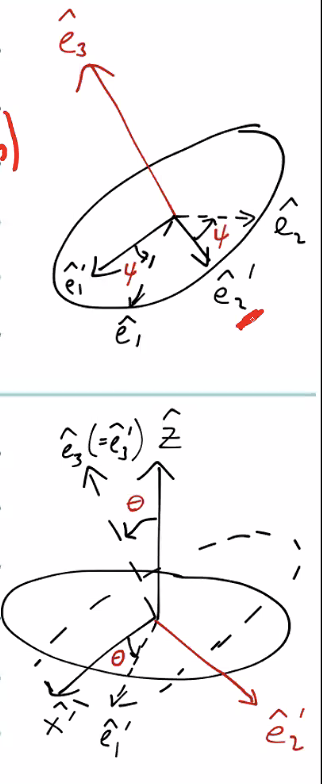
\includegraphics[scale=0.5]{Lecture-21/l21-img1.png}
\end{center}
We will use the Euler angles to get the general Lagrangian. Recall that $T = \frac{1}{2}\bm{\omega}\cdot\v{L}$. Using Euler Angles, we have:
\[\bm{\omega} = \dot{\phi}\zhat + \dot{\theta}\hat{\v{e}}_2' + \dot{\psi}\hat{\v{e}}_3\]
this is the vector sum of these three components, each of which are written in a different coordinate system (related by rotations). We will now expand this in the body frame. We know that:
\[\hat{\v{e}}_2' = R_{e3}\hat{\v{e}}_2 = \m{\cos\psi & \sin\psi & 0 \\ -\sin\psi & \cos\psi & 0 \\ 0 & 0 & 1}\m{0 \\ 1 \\ 0} = \sin\psi\hat{\v{e}}_1 + \cos\psi\hat{\v{e}}_2 \]
In a similar way, we get:
\[\hat{\v{e}}_1' = \cos\psi\hat{\v{e}}_1 - \sin\psi\hat{\v{e}}_2\]
Note that this is a passive transformation. Next, we determine:
\[\zhat = R_{e2'}\hat{\v{e}}_3 = \m{\cos\theta & 0 & -\sin\theta \\ 0 & 1 & 0 \\ \sin\theta & 0 & \cos\theta}\m{0 \\ 0 \\1} = -\sin\theta\hat{\v{e}}_1' + \cos\theta\hat{\v{e}}_3' = -\sin\theta\cos\psi\hat{\v{e}}_1 + \sin\theta\sin\psi\hat{\v{e}}_2 + \cos\theta\hat{\v{e}}_3\]
Therefore plugging back into the original equation and collecting the terms, we get:
\[\bm{\omega} = (\dot{\theta}\sin\psi - \dot{\phi}\sin\theta\cos\psi)\hat{\v{e}}_1 + (\dot{\theta}\cos\psi+\dot{\phi}\sin\theta\sin\psi)\hat{\v{e}}_2 + (\dot{\phi}\cos\theta + \dot{\psi})\hat{\v{e}}_3\]
Therefore, in the body frame, the kinetic energy is easy to calculate (as the inertia tensor is diagonal) so:
\[T = \frac{1}{2}\left(\lambda_1\omega_1^2 + \lambda_2\omega_2^2 + \lambda_3\omega_3^2\right) = \frac{\lambda_1}{2}(\dot{\theta}^2 + \dot{\phi}^2\sin^2\theta) + \frac{\lambda_3}{2}(\dot{\psi} + \dot{\phi}\cos\theta)^2 \]
Where we suppose that $\lambda_1 = \lambda_2$ as the top is symmetric.

\noindent Question: How does the kinetic energy in the body frame $T = \frac{1}{2}\bm{\omega} \cdot \II \bm{\omega}$ compare to the kinetic energy in the space frame?
\begin{s}
We will come back to this on Wednesday. Try a conversion between the two frames by a rotation and see what you get.
\end{s}

\subsubsection{Symmetry Spinning Top with Torque (Gravity)}
\begin{center}
    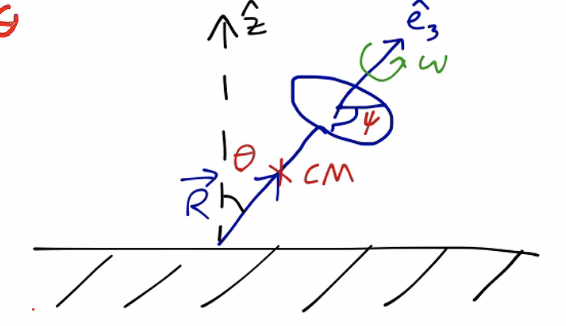
\includegraphics[scale=0.5]{l21-img2.png}
\end{center}
Now, we consider a spinning top with gravity. We have that the Lagrangian gives:
\[\LL = \frac{1}{2}\left[\lambda_3\left(\dot{\psi} + \dot{\phi}\cos\theta\right)^2 + \lambda_1\left(\dot{\phi}^2\sin^2\theta + \dot{\theta}^2\right)\right] - mgR\cos\theta\]
From which we can see that the total energy, the generalized momentum associated with $\psi$, and the generalized momentum associated with $\phi$ are conserved (The Lagrangian does not depend on $\psi$ or $\phi$, so they are cyclic and conserved). Calculating $p_\psi$, we get:
\[p_\psi = \dpd{\LL}{\dot{\psi}} = \lambda_3(\dot{\psi} + \dot{\phi}\cos\theta) = \lambda_3\omega_3 = L_3 = C\]
Which is just the angular momentum in the e3 direction in the body frame. Doing the same for $p_\phi$, we have:
\[p_{\phi} = \dpd{\LL}{\dot{\phi}} = \lambda_1\dot{\phi}\sin^2\theta + \lambda_3(\dot{\phi}\cos\theta + \dot{\psi})\cos\theta = L_z = C\]
Which is the z-component of the angular momentum in the space frame, which makes sense if we think about the effects of gravity. Finally, we calculate the equation for $\theta$ (which is the only quantity that can evolve:
\[\lambda_1\ddot{\theta} = \lambda_1\dot{\phi}^2\sin\theta\cos\theta - \lambda_3\dot{\phi}\sin\theta(\dot{\psi} + \dot{\phi}\cos\theta) + MgR\sin\theta\]
Now, we consider the simple situation where $\theta$ is constant. Then, $\dot{\theta} = \ddot{\theta} = 0$, and from the equations for $\dot{\phi}$ and $\dot{\psi}$ we see that the also are constant. Then, let us call $\dot{\phi} = \Omega$. Writing the EOM for $\theta$, we have:
\[0 = \lambda_1\Omega^2\cos\theta - \lambda_3\Omega\omega_3 + MgR\]
This is a quadratic equation for $\Omega$, from which we can solve for it. For $\omega_3$ large, we get two solutions:
\[\Omega_1 \approx \frac{\lambda_3\omega_3}{\lambda_1\cos\theta}\]
Which is actually independent of $g$! It is the same precession we saw for the free top. The other frequency is given by:
\[\Omega_2 \approx \frac{MgR}{\lambda_3\omega_3}\]
Which is precession due to the gravitational torque. 

\end{document}


